%%%%%%%%%%%%%%%%%%%%%%%%%%%%%%%%%%%%%%%%%
% Structured General Purpose Assignment
% LaTeX Template
%
% This template has been downloaded from:
% http://www.latextemplates.com
%
% Original author:
% Ted Pavlic (http://www.tedpavlic.com)
%
% Note:
% The \lipsum[#] commands throughout this template generate dummy text
% to fill the template out. These commands should all be removed when 
% writing assignment content.
%
%%%%%%%%%%%%%%%%%%%%%%%%%%%%%%%%%%%%%%%%%

%----------------------------------------------------------------------------------------
%	PACKAGES AND OTHER DOCUMENT CONFIGURATIONS
%----------------------------------------------------------------------------------------

\documentclass{article}

\usepackage{fancyhdr} % Required for custom headers
\usepackage{lastpage} % Required to determine the last page for the footer
\usepackage{extramarks} % Required for headers and footers
\usepackage{graphicx} % Required to insert images
\usepackage{lipsum} % Used for inserting dummy 'Lorem ipsum' text into the template
\usepackage{amsfonts}
\usepackage{subfig}
\usepackage{graphicx}
\usepackage{caption}
\usepackage{amsmath}
\usepackage{forest}
\usepackage{float}
\usepackage{listings}
\usepackage{hyperref}


%----------------------------------------------------------------------------------------
%	NAME AND CLASS SECTION
%----------------------------------------------------------------------------------------

\newcommand{\hmwkTitle}{Assignment\ \#1} % Assignment title
\newcommand{\hmwkDueDate}{Sunday,\ April\ 17,\ 2016} % Due date
\newcommand{\hmwkClass}{CS\ 254} % Course/class
\newcommand{\hmwkClassInstructor}{Prof. Tim Sherwood} % Teacher/lecturer
\newcommand{\hmwkAuthorName}{Chad Spensky} % Your name

%----------------------------------------------------------------------------------------
%	TITLE PAGE
%----------------------------------------------------------------------------------------

\title{
\vspace{2in}
\textmd{\textbf{\hmwkClass:\ \hmwkTitle}}\\
\normalsize\vspace{0.1in}\small{Due\ on\ \hmwkDueDate}\\
\vspace{0.1in}\large{\textit{\hmwkClassInstructor}}
\vspace{3in}
}

\author{\textbf{\hmwkAuthorName}}
\date{} % Insert date here if you want it to appear below your name

%----------------------------------------------------------------------------------------

\begin{document}

\maketitle
\newpage

\newcommand{\fancyx}{\ensuremath{ \mathcal{X}}}
\newcommand{\fancyy}{\ensuremath{ \mathcal{Y}}}


\newcommand*{\QED}{\hfill\ensuremath{\square}}%


%----------------------------------------------------------------------------------------
%	TABLE OF CONTENTS
%----------------------------------------------------------------------------------------

%\setcounter{tocdepth}{1} % Uncomment this line if you don't want subsections listed in the ToC
%
%\newpage
%\tableofcontents
%\newpage

% To have just one problem per page, simply put a \clearpage after each problem

\section{Branches (2pts)}
\subsection{Bimodal Predictor}
In this case, we first want to prime the predictor to the \emph{not branch case}, and which point we want to branch every other case
\lstinputlisting[language=C]{bimodal.c}

See the output below:\\
\begin{tabular}{| l | l | l | l |}
\hline
  \bf{i} & \bf{Predictor Value} & \bf{Branch Prediction} & \bf{Branch Condition} \\\hline
  1 & 0b?? & ? & False \\\hline
  2 & 0b?? & ? & False \\\hline
  3 & 0b?? & Not taken & False \\\hline
  4 & 0b00 & Not taken & True \\\hline
  5 & 0b01 & Not taken & True \\\hline
  6 & 0b10 & Taken & False \\\hline
  7 & 0b01 & Not taken & True \\\hline
  \dots & \dots & \dots & \dots \\\hline
\end{tabular}
  
\subsection{Modified Bimodal Predictor (Hennessey and Patterson)}
In this case, we first want to prime the predictor to the \emph{not branch case}, and which point we want do 3 instances where we don't take the branch to load up the predictor, then 3 instances where we do take the branch, and continuously repeat this.
\lstinputlisting[language=C]{bimodal_2.c}

See the output below:\\
\begin{tabular}{| l | l | l | l |}
\hline
  \bf{i} & \bf{Predictor Value} & \bf{Branch Prediction} & \bf{Branch Condition} \\\hline
  1 & 0b?? & ? & False \\\hline
  2 & 0b?? & ? & False \\\hline
  3 & 0b?? & Not taken & False \\\hline
  4 & 0b00 & Not taken & True \\\hline
  5 & 0b00 & Not taken & True \\\hline
  6 & 0b00 & Not taken (S-Not, S-Not, S-Not) & True \\\hline
  7 & 0b01 & Not taken (S-Not, S-Not, W-Not)  & True \\\hline
  8 & 0b10 & Not taken (S-Not, W-Not, W-Taken) & True \\\hline
  9 & 0b11 & Taken (W-Not, W-Taken, S-Taken)& False \\\hline
  10 & 0b10 & Taken (W-Taken, S-Taken, W-Taken) & False \\\hline
  11 & 0b01 & Taken (S-Taken, W-Taken, W-Not) & False \\\hline
  12 & 0b00 & Not taken (W-Taken, W-Not, S-Not) & True \\\hline
  \dots & \dots & \dots & \dots \\\hline
\end{tabular}
  
\newpage
 
\section{Instruction Level Parallelism (2pts)}
\subsection{A (Scalar, in-order, cache misses stall)}
In this case, we have a very straightforward analysis where all instructions are 1 cycle and loads are expected to take $.3*1 + .7*10 = 7.3$ cycles since cache hits (30\% of the time) are only 1 cycle and misses (70\% of the time) take 10 cycles.

Thus, the IPC is simply the number of instructions divided by the number of cycles taken for the loop. 
More precisely,
\begin{equation*}
IPC = \frac{7~ins}{2*(.3*1+.7*10) +5)~cycles} \approx 0.36~ins/cycle
\end{equation*}


\subsection{B (2-way super scalar, in-order, no cache misses)}
In this case, all instructions will only take two cycles and two instructions be executed together $\iff$ they have no dependencies.  Unfortunately this only happens with the instructions at $0x14$ and $0x18$, permitting the execution of 2 instructions in that cycle.

Thus
\begin{equation*}
IPC = \frac{7~ins}{6~cycles} \approx 1.17~ins/cycle
\end{equation*}

\subsection{C (2-way super scalar, in-order, cache misses stall)}
Since neither of the superscalar instructions are loads, our new equations is effectively:
\begin{equation*}
IPC = \frac{7~ins}{2*(.3*1+.7*10) +4)~cycles} \approx 0.38~ins/cycle
\end{equation*}

\subsection{D (Scalar, out-of-order, infinite renaming, infinite ALUS, no cache misses)}
In this case we would expect an instruction to execute at every cycle, giving us 1 instruction per cycle.  This is because of our perfect branch prediction.  That would enable the machine to always schedule around data-dependencies and start computing the next loop.  If this were a 2-way super scalar machine, it could achieve 2 instructions per cycle.

\subsection{E (Scalar, out-of-order, infinite renaming, infinite ALUS, no cache misses)}
In this case, we would expect the same outcome as before, where could achieve 1 instruction per cycle.

\newpage

\section{Combining Branch Predictions (10pts)}
All of these predictors were implemented in python, the results are below:
{\footnotesize
\begin{tabular}{| r | c | c | c |}
\hline
   & \bf{Global Predictor} & \bf{Local Predictor} & \bf{Tournament Predictor} \\\hline
Correct Predictions 	& 3414883 (89.584659\%)		& 2519412 (66.093235\%)		& 3532738 (92.676420\%) \\\hline
Missed Predictions 	& 397023 (10.415341\%)		& 1292494 (33.906765\%)		& 279168 (7.323580\%) \\\hline
Most-missed PC 	& 0x40141c69 (23918 times)	& 0xa0edf91b (152601 times)	& 0x40141c69 (24755 times)\\
\hline
\end{tabular}
}

\newpage

\section{Pipelines and Branch Prediction (6pts)}
In this problem, we need to incorporate R into our execution time speedup equation:
\begin{equation*}
ET = \frac{time}{cycle} + \frac{cycle}{instructions} + \frac{instructions}{program}
\end{equation*}
which as a speedup is:
\begin{equation*}
ET_{speedup} = \frac{\frac{S_0}{C_0}}{\frac{S_n}{C_n}} * \frac{\frac{C_0}{I_0}}{\frac{C_n}{I_n}} * \frac{\frac{I_0}{I_0}}{\frac{I_n}{P_n}}
\end{equation*}

Since we aren't changing the cycles, instructions, or program, the right 2 portions of the equation remain the same (in fact, instructions per program is unchanged):
\begin{equation*}
ET_{speedup} = \frac{\frac{S_0}{C_0}}{\frac{S_n}{C_n}} * \frac{1}{1+\frac{P}{B}}*1
\end{equation*}
$S_0$ is $W$ and $C_0$ remains unchanged.  $C_n = C_0*P$ since we are now increasing the total number of cycles per second.  Similarly, the time taken now is $S_n = W+RP$.  Thus, our new equation is:
\begin{eqnarray*}
ET_{speedup} & = \frac{\frac{W}{C_0}}{\frac{W+R*P}{C_0*P}} * \frac{1}{1+\frac{P}{B}}\\
& = \frac{WP}{W+R*P} * \frac{1}{1+\frac{P}{B}}
\end{eqnarray*}
So for $W=1ns, R=100ps, B = 100$, we get:
\begin{eqnarray*}
ET_{speedup} & = \frac{P}{1+\frac{P}{100}} * \frac{1}{1+\frac{P}{100}}\\
& = \frac{1+P}{(1+\frac{P}{100})^2}
\end{eqnarray*}
which has the derivative of:
\begin{equation*}
-\frac{10,000(P-100)} {(P+100)^3}
\end{equation*}
Implying that our maximum value will be achieved at $\mathbf{P = 100}$.
\newpage
To solve this generally, one could calculate the derivative of the base equation.  However, it has been a while since I've done this level of calculus, and my memory is a little shady on it.  Neverthless, Wolfram Alpha does offer some insights: \url{https://www.wolframalpha.com/input/?i=derivative+WP\%2F(W\%2BRP)\%2B1\%2F(1\%2BP\%2FB)}
Finding the roots of this equation would provide potential maxima:\\
\begin{figure}
\centering
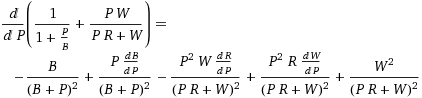
\includegraphics[width=.8\textwidth]{derivative.png}
%\end{homeworkProblem}
\end{figure}
\end{document}